
\documentclass[12pt]{article}

\usepackage{amsmath, mathtools}
\usepackage{amsfonts}
\usepackage{amssymb}
\usepackage{graphicx}
\usepackage{colortbl}
\usepackage{xr}
\usepackage{hyperref}
\usepackage{longtable}
\usepackage{xfrac}
\usepackage{tabularx}
\usepackage{float}
\usepackage{siunitx}
\usepackage{booktabs}
\usepackage{caption}
\usepackage{pdflscape}
\usepackage{afterpage}

\usepackage[round]{natbib}

%\usepackage{refcheck}

\hypersetup{
    bookmarks=true,         % show bookmarks bar?
      colorlinks=true,       % false: boxed links; true: colored links
    linkcolor=red,          % color of internal links (change box color with linkbordercolor)
    citecolor=green,        % color of links to bibliography
    filecolor=magenta,      % color of file links
    urlcolor=cyan           % color of external links
}

% For easy change of table widths
\newcommand{\colZwidth}{1.0\textwidth}
\newcommand{\colAwidth}{0.13\textwidth}
\newcommand{\colBwidth}{0.82\textwidth}
\newcommand{\colCwidth}{0.1\textwidth}
\newcommand{\colDwidth}{0.05\textwidth}
\newcommand{\colEwidth}{0.8\textwidth}
\newcommand{\colFwidth}{0.17\textwidth}
\newcommand{\colGwidth}{0.5\textwidth}
\newcommand{\colHwidth}{0.28\textwidth}

% Used so that cross-references have a meaningful prefix
\newcounter{defnum} %Definition Number
\newcommand{\dthedefnum}{GD\thedefnum}
\newcommand{\dref}[1]{GD\ref{#1}}
\newcounter{datadefnum} %Datadefinition Number
\newcommand{\ddthedatadefnum}{DD\thedatadefnum}
\newcommand{\ddref}[1]{DD\ref{#1}}
\newcounter{theorynum} %Theory Number
\newcommand{\tthetheorynum}{T\thetheorynum}
\newcommand{\tref}[1]{T\ref{#1}}
\newcounter{tablenum} %Table Number
\newcommand{\tbthetablenum}{T\thetablenum}
\newcommand{\tbref}[1]{TB\ref{#1}}
\newcounter{assumpnum} %Assumption Number
\newcommand{\atheassumpnum}{P\theassumpnum}
\newcommand{\aref}[1]{A\ref{#1}}
\newcounter{goalnum} %Goal Number
\newcommand{\gthegoalnum}{P\thegoalnum}
\newcommand{\gsref}[1]{GS\ref{#1}}
\newcounter{instnum} %Instance Number
\newcommand{\itheinstnum}{IM\theinstnum}
\newcommand{\iref}[1]{IM\ref{#1}}
\newcounter{reqnum} %Requirement Number
\newcommand{\rthereqnum}{P\thereqnum}
\newcommand{\rref}[1]{R\ref{#1}}
\newcounter{nfrnum} %NFR Number
\newcommand{\rthenfrnum}{NFR\thenfrnum}
\newcommand{\nfrref}[1]{NFR\ref{#1}}
\newcounter{lcnum} %Likely change number
\newcommand{\lthelcnum}{LC\thelcnum}
\newcommand{\lcref}[1]{LC\ref{#1}}
\newcounter{ucnum} %Likely change number
\newcommand{\ltheucnum}{LC\theucnum}
\newcommand{\ucref}[1]{UC\ref{#1}}

\usepackage{fullpage}

\newcommand{\deftheory}[9][Not Applicable]
{
\newpage
\noindent \rule{\textwidth}{0.5mm}

\paragraph{RefName: } \textbf{#2} \phantomsection 
\label{#2}

\paragraph{Label:} #3

\noindent \rule{\textwidth}{0.5mm}

\paragraph{Equation:}

#4

\paragraph{Description:}

#5

\paragraph{Notes:}

#6

\paragraph{Source:}

#7

\paragraph{Ref.\ By:}

#8

\paragraph{Preconditions for \hyperref[#2]{#2}:}
\label{#2_precond}

#9

\paragraph{Derivation for \hyperref[#2]{#2}:}
\label{#2_deriv}

#1

\noindent \rule{\textwidth}{0.5mm}

}

\begin{document}


\title{Software Requirements Specification for Solar Cooker Energy Calculator: A Software for calculating heat loss and observed heat} 
\author{Deesha Patel}
\date{\today}
	
\maketitle

~\newpage

\pagenumbering{roman}

\tableofcontents

~\newpage

\section*{Revision History}

\begin{tabularx}{\textwidth}{p{3cm}p{2cm}X}
\toprule {\bf Date} & {\bf Version} & {\bf Notes}\\
\midrule
02/04/2023 & 0.1 & Initial Release\\
02/11/2023 & 0.2 & Update document for first 4 issues \\ 
02/11/2023 & 0.3 & Update document for 5 to 9 issues \\ 
02/11/2023 & 0.4 & All changes done \\
\bottomrule
\end{tabularx}

~\newpage

\section{Reference Material}

This section records information for easy reference.

\subsection{Table of Units}

Throughout this document SI (Syst\`{e}me International d'Unit\'{e}s) is employed
as the unit system.  In addition to the basic units, several derived units are
used as described below.  For each unit, the symbol is given followed by a
description of the unit and the SI name.
~\newline

\renewcommand{\arraystretch}{1.2}
%\begin{table}[ht]
  \noindent \begin{tabular}{l l l} 
    \toprule		
    \textbf{symbol} & \textbf{unit} & \textbf{SI}\\
    \midrule 
    \si{\metre} & length & metre\\
    \si{\kilogram} & mass	& kilogram\\
    \si{\second} & time & second\\
    \si{\celsius} & temperature & centigrade\\
    \si{\joule} & energy & joule\\
    \si{\watt} & power & watt (W = \si{\joule\per\second})\\
    \bottomrule
  \end{tabular}
  %	\caption{Provide a caption}
%\end{table}

\subsection{Table of Symbols}

The table that follows summarizes the symbols used in this document along with
their units.  The choice of symbols was made to be consistent with the heat
transfer energy.  The symbols are listed in alphabetical order.

\renewcommand{\arraystretch}{1.2}
%\noindent \begin{tabularx}{1.0\textwidth}{l l X}
\noindent \begin{longtable*}{l l p{12cm}} \toprule
\textbf{symbol} & \textbf{unit} & \textbf{description}\\
\midrule 

$A_\text{g}$ & \si[per-mode=symbol] {\square\metre} & Area of glass
\\ 

$A_\text{m}$ & \si[per-mode=symbol] {\square\metre} & Wet surface area over which heat is transferred in
\\ 

$A_r$ & \si[per-mode=symbol] {\square\metre} & Area of Reflector
\\

$A_t$ & \si[per-mode=symbol] {\square\metre} & Area of Lid 
\\


$A_\text{ref}$ & $\si[per-mode=symbol] {\square\metre} $ & Reflector area with respect to different reflectors \\

$C$ & $\si{\joule\per(\kilogram \celsius)}$ & Specific Heat Capacity of material \\

$C_W$ & $\si{\joule\per(\kilogram \celsius)}$ & Specific Heat Capacity of Water \\

$E_W$ & $\si{\joule}$ & Change in heat energy in the Water \\

$f$ & - & Fluid \\

$G$ & \si[per-mode=symbol]{\watt\per\square\metre} & Incidental solar radiation \\

$g_1$ & - & Glass 1\\

$g_2$ & - & Glass 2 \\

$h$ & \si[per-mode=symbol]{\watt\per\square\metre K} & Heat transfer convection coefficient \\

$int1$ & - & Inner part between glass 1 and glass 2 \\

$int2$ & - & Inner part of the solar cooker box \\

$int3$ & - & Inner part of container \\

$L$ & \si{\metre} & Length of box \\

$m_W$ & \si{\kilogram} & Mass of Water \\

$n$ & - & Number of Reflector \\

$q$ & \si{\watt\per\square\metre} & Thermal flux vector \\

$Q$ & \si{\watt} & Quantity of heat transfer to or from the object \\

$r$ & - & Recipient \\

$ref$ & - & Reflector \\

$T$ & \si{\celsius} & Temperature\\

$T_W$ & \si{\celsius} & Temperature of Water\\

$t$ & - & Lid of recipient\\

$\epsilon$ & \si{\mu}m & Emittance \\

$\tau$ & \si[per-mode=symbol]{\watt\per\square\metre K} & Transmittivity \\

$\theta$ & radians & Reflector Angle \\ 

$\sigma$ & \si[per-mode=symbol]{\watt\per\square\metre K^4} & Steffan-Boltzman constant \\

$\rho$ & \si{\kilogram\per\metre^3} & Reflectivity \\

\bottomrule
\end{longtable*}

\subsection{Abbreviations and Acronyms}

\renewcommand{\arraystretch}{1.2}
\begin{tabular}{l l} 
  \toprule		
  \textbf{symbol} & \textbf{description}\\
  \midrule 
  A & Assumption\\
  DD & Data Definition\\
  GD & General Definition\\
  GS & Goal Statement\\
  IM & Instance Model\\
  LC & Likely Change\\
  PS & Physical System Description\\
  R & Requirement\\
  SRS & Software Requirements Specification\\
  T & Theoretical Model\\
  \bottomrule
\end{tabular}\\

\newpage

\pagenumbering{arabic}

\section{Introduction}

As fossil fuels adversely affect the environment, many countries like India, where they have good solar rays throughout the year, have started to implement devices for utilizing solar energy and transforming it into valuable energy. It includes solar water heaters, solar panels, and solar cookers. It is indeed a fact that the demand for renewable energy has increased to deal with the problem of limited non-renewable resources. Focusing on the Solar Cooker, several designs such as the Solar Panel Cooker, Solar Parabolic Cooker, and Solar Box Cooker have been proposed to utilize more solar energy. Using internal reflectors, we would like to improve the utilization of solar energy during cooking food.   

The following section provides an overview of the Software Requirement Specification (SRS) for a box-type Solar Cooker. This section explains the purpose of the document, the scope of requirements, the characteristics of the intended reader, and the organization of the document.   


\subsection{Purpose of Document}

We are going to use the Solar Box Cooker in this software. The main purpose of this document is to describe a mathematical model of a Solar Cooker~\cite{MathsModel} which can provide a calculation for internal reflector in solar box that can help to improve the temperature in the box with a variety of parameters that attempts to define the intended functionality required. Thus, this document provides detailed requirements of the software which will be used in planing for design stage. Therefore, this document is intended to be used as a reference to provide ad hoc access to all information necessary to understand and verify the model. This document describes goals, assumptions, theoretical models, and important definitions to understand the problem. The SRS is abstract because the content here says \emph{what} the problem is. But it does not say anything related to \emph{how} to solve it.

\subsection{Scope of Requirements} 

Numerous algorithms have been analyzed for the efficiency of a Solar Cooker. The scope of the requirement includes a mathematical model to determine the thermal function of a box-type solar cooker with an internal reflectors. With the help of different inputs, this system calculates the achieved temperature by implementing the proposed solution. However, this project not focusing on more than one iteration for the reflections. In other words, this project focuses on the reflection from glass 2 to recipient.   

\subsection{Characteristics of Intended Reader} \label{sec_IntendedReader}

Firstly, Intended Reader or Reviewer should have knowledge of heat transfer theory and radiant solar energy. A person should have completed a Heat Transfer course during their bachelor of engineering (Mechanical Engineering and Chemical Engineering expected). A reader should have knowledge about the differential equation; offered in the second year Calculus course.        

\subsection{Organization of Document}

The organization of this document follows the template for an SRS for scientific 
computing software proposed by~\cite{Koothoor2013} and \cite{SmithAndLai2005}.
The presentation follows the standard pattern of presenting goals, theories, definitions, 
and assumptions. For readers that would like a more bottom up approach, they can start 
reading the instance models in Section~\ref{sec_instance} and trace back to find any 
additional information they require. The goal statements are refined to the theoretical models, 
and the theoretical models to the instance models. The instance model 
(Section~\ref{sec_instance}) to be solved is referred to as \iref{ewat}.

\section{General System Description}

This section provides general information about the system.  It identifies the
interfaces between the system and its environment, describes the user
characteristics and lists the system constraints.  

\subsection{System Context}

The system context is shown in Figure \ref{Fig_SystemContext} below. The circles represent the user, who is both responsible for handling the inputs and the outputs. The box represents the program itself, and the arrows indicate what data and information is passed between the user and the program. 

\begin{figure}[h!]
\begin{center}
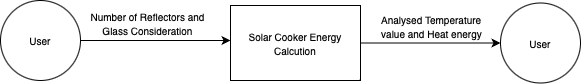
\includegraphics[width=0.6\textwidth]{SystemContext}
\caption{System Context}
\label{Fig_SystemContext} 
\end{center}
\end{figure}

\begin{itemize}
\item User Responsibilities:
\begin{itemize}
\item Provide required inputs including number of reflectors, glass area, thickness, dimension and size. 
\item Ensure all inputs are in correct format. 
\end{itemize}

\item Software Responsibilities:
\begin{itemize}
\item Detect data type mismatch, such as a string of characters instead of a
  floating point number
\item Determine if the inputs satisfy the required physical and software constraints such as thickness of the glass is not negative value
\item Calculate and plot the required outputs of temperature
\end{itemize}
\end{itemize}

\subsection{User Characteristics} \label{SecUserCharacteristics}

The end user of the system is expected to be familiar with undergraduate level Calculus and basic Physics. They should also know basics about the reflector angle and heat flows in solar cooker.  

\subsection{System Constraints}

There are no system constraints for this project.

\section{Specific System Description}

This section first presents the problem description, which gives a high-level
view of the problem to be solved.  This is followed by the solution characteristics
specification, which presents the assumptions, theories, definitions and finally
the instance models (ODE) that models the Solar Cooker Reflections.

\subsection{Problem Description} \label{Sec_pd}

Solar Cooker Energy Calculation is intended to investigate the temperature inside the solar cooker box with internal reflectors. 

\subsubsection{Terminology and  Definitions}

This subsection provides a list of terms that are used in the subsequent
sections and their meaning, with the purpose of reducing ambiguity and making it
easier to correctly understand the requirements:

\begin{itemize}

\item Reflectivity: The fraction of radiation reflected by the surface is called the reflectivity ($\rho$). 
\item Transmittivity: The fraction of radiation transmitted is called the transmissivity ($\tau$).
\item Emittance: The energy radiated by the surface of a body per second per unit area ($\epsilon$).
\item Reflactor Angle: The angle between a reflected ray and the normal drawn at the point of incidence to a reflecting surface ($\theta$).
\item Heat flow Convection: Convection is the transfer of heat from one place to another due to the movement of fluid. 
\item Heat flow radiation: A process where heat waves are emitted that may be absorbed, reflected, or transmitted through a colder body.
\item Heat Convection Coefficients: The rate of heat transfer between a solid surface and a fluid per unit surface area per unit temperature difference (h). 
\item Steffan-Boltzman constant: A physical constant expressing the relationship between the heat radiation emitted by a black body and its absolute temperature ($\sigma$).
\item Heat/Thermal Flux: The amount of heat energy passing through a certain surface.
\item Heat Capacity: Heat capacity or thermal capacity is a physical property of matter, defined as the amount of heat to be supplied to an object to produce a unit change in its temperature. 
\item Incidental Solar Radiation: The amount of solar radiation that hits the earth’s surface per unit of time and area. 


\end{itemize}

\subsubsection{Physical System Description} \label{sec_phySystDescrip}

The physical system of Solar Cooker
Energy Calculation, as shown in Figure \ref{Fig_HeatFlows},
includes the following elements:


\begin{itemize}

\item[PS1:] A cover with two flat glasses (glass 1 and glass 2) 

\item[PS2:] Lead of the recipient 

\item[PS3:] Recipient itself

\item[PS4:] Fluid inside the recipient

\end{itemize}

\begin{figure}[h!]
\begin{center}
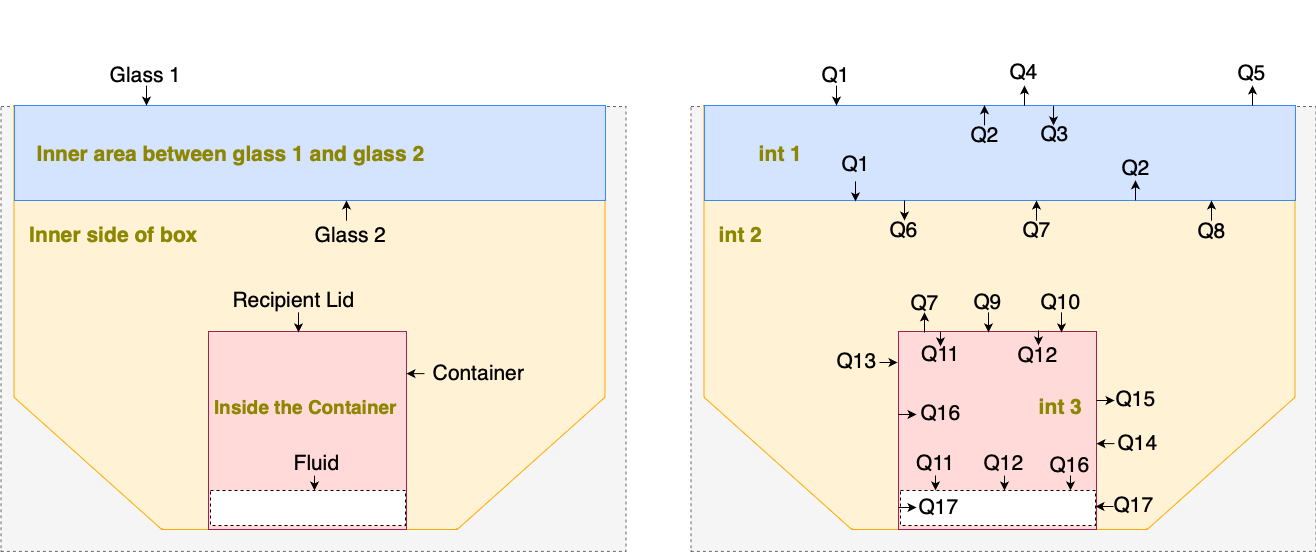
\includegraphics[width=0.90\textwidth]{HeatFlow}
\caption{Heat Flows in Solar Cooker}
\label{Fig_HeatFlows} 
\end{center}
\end{figure}


% \begin{figure}[h!]
% \begin{center}
% %\rotatebox{-90}
% {
%  \includegraphics[width=0.5\textwidth]{<FigureName>}
% }
% \caption{\label{<Label>} <Caption>}
% \end{center}
% \end{figure}

\subsubsection{Goal Statements}

\noindent Given the thermal attributes, solar box characteristics and initial conditions the goal statements are:

\begin{itemize}

\item[GS\refstepcounter{goalnum}\thegoalnum \label{G_meaningfulLabel}:] predicts the temperature over the recipient (a cooking container).

\item[GS\refstepcounter{goalnum}\thegoalnum \label{G_meaningfulLabel}:] predicts the temperature of the fluid (a water inside the container).

\item[GS\refstepcounter{goalnum}\thegoalnum \label{G_meaningfulLabel}:] predicts the cooking energy in the recipient over time.

\end{itemize}

\subsection{Solution Characteristics Specification}

The instance model (ODE) that governs Solar Cooker
Energy Calculator is presented in
Subsection~\ref{sec_instance}.  The information to understand the meaning of the
instance model and its derivation is also presented, so that the instance
model can be verified.

\subsubsection{Assumptions} \label{sec_assumpt}


This section simplifies the original problem and helps in developing the
theoretical model by filling in the missing information for the physical
system. The numbers given in the square brackets refer to the theoretical model
[T], general definition [GD], data definition [DD], instance model [IM], or
likely change [LC], in which the respective assumption is used.

\begin{itemize}

\item[A\refstepcounter{assumpnum}\theassumpnum \label{A_1}:] The emissivity(\si{\epsilon}) is constant. [\dref{HFC}, \ddref{dd_q_12} , \ddref{dd_q_15}, \ddref{dd_q_16}, \iref{ewat}] 

\item[A\refstepcounter{assumpnum}\theassumpnum \label{A_2}:] The reflectivity (\si{\rho}) is constant. [\ddref{dd_q_14}]

\item[A\refstepcounter{assumpnum}\theassumpnum \label{A_3}:] The Transmisivity (\si{\tau}) is constant. [\ddref{dd_q_14}]

\item[A\refstepcounter{assumpnum}\theassumpnum \label{A_4}:] The material in the recipient (Container) is water. [\iref{ewat}, \tref{TM_2}] 

\item[A\refstepcounter{assumpnum}\theassumpnum \label{A_5}:]The  temperature of water will not drop below melting point. [\iref{ewat}, \tref{TM_2}]  

\item[A\refstepcounter{assumpnum}\theassumpnum \label{A_6}:]The temperature of water will not rise above the boiling point. [\iref{ewat}, \tref{TM_2}]   

\item[A\refstepcounter{assumpnum}\theassumpnum \label{A_7}:] The temperature $T_\text{int2}$ (temperature inside the box) are obtained by calculating mean of temperature value of inner glass ($g_2$), lid of the recipient, and reflector. [\iref{ewat}, \ddref{dd_q_13}] 

\item[A\refstepcounter{assumpnum}\theassumpnum \label{A_8}:] The temperature $T_\text{int3}$ (temperature inside the container) are obtained by calculating mean of temperature of lid and fluid. [\iref{im2}, \ddref{dd_q_11}]


\item[A\refstepcounter{assumpnum}\theassumpnum \label{A_9}:] The solar radiation impact over the solar cooker occurs in perpendicular way. [\iref{ewat}, \ddref{dd_q_14}] 

\item[A\refstepcounter{assumpnum}\theassumpnum \label{A_10}:] The only form of energy considered in this problem is thermal energy. Other energy such as mechanical energy are assumed to be a negligible. [\iref{ewat}, \lcref{LC_1}] 


\end{itemize}

\newpage

\subsubsection{Theoretical Models}\label{sec_theoretical}

This section focuses on the general equations and laws that Solar Cooker
Energy Calculator is based
on.

~\newline

\noindent
\begin{minipage}{\textwidth}
\renewcommand*{\arraystretch}{1.5}
\begin{tabular}{| p{\colAwidth} | p{\colBwidth}|}
  \hline
  \rowcolor[gray]{0.9}
  Number& TM\refstepcounter{theorynum}\thetheorynum \label{TM_1}\\
  \hline
  Label& \bf Convective Heat Transfer Coefficient\\
  \hline
  Equation &
    $h = \frac{q}{\triangle T}$ \\ 
  \hline
  Description
    & The above equation is used to calculate the heat transfer typically by convection or phase transition.  \\
  
   & $h$ is the heat transfer convection coefficient $(\si[per-mode=symbol] {\watt\per\square\metre} K).$  \\
  
  & $q$ is the thermal flux vector $(\si{\watt\per\square\metre} )$.  \\
  
  & $\triangle$T is the change in temperature. \\
  \hline
  Notes & none. \\
  \hline
  Sources& \url{https://en.wikipedia.org/wiki/Heat_transfer_coefficient} \\
  \hline
  Ref.\ By &  \dref{HFC}, \iref{ewat} \\
  \hline
\end{tabular}
\end{minipage}\\
~\newline

\noindent
\begin{minipage}{\textwidth}
\renewcommand*{\arraystretch}{1.5}
\begin{tabular}{| p{\colAwidth} | p{\colBwidth}|}
  \hline
  \rowcolor[gray]{0.9}
  Number& TM\refstepcounter{theorynum}\thetheorynum \label{TM_2}\\
  \hline
  Label& \bf Sensible Heat energy Calculation\\
  \hline
  Equation &
    $Q = Cm \triangle T$ \\ 
  \hline
  Description
    & This calculation occurs until the highest or lowest temperature reach, as assumed in [\aref{A_4}] \\
  & $Q$ is the quantity of heat in the object \\ 
  & $m$ is the mass of the object \\ 
 & $C$ is the specific heat capacity of the material the object is composed of \\ 
  & $\si{\triangle} T$ is the temperature change of the object   \\
  
  \hline
  Notes & none. \\
  \hline
  Sources& \url{https://www.physicsclassroom.com/class/thermalP/Lesson-2/Measuring-the-Quantity-of-Heat} \\
  \hline
  Ref.\ By &  \iref{I_HETR}\\
  \hline
\end{tabular}
\end{minipage}\\


~\newline


\noindent
\begin{minipage}{\textwidth}
\renewcommand*{\arraystretch}{1.5}
\begin{tabular}{| p{\colAwidth} | p{\colBwidth}|}
  \hline
  \rowcolor[gray]{0.9}
  Number& TM\refstepcounter{theorynum}\thetheorynum \label{TM_3}\\
  \hline
  Label& \bf Conservation of thermal energy\\
  \hline
  Equation &
      $-{\bf \nabla \cdot q} + g$ = $\rho C \frac{\partial T}{\partial t}$ \\ 
  \hline
  Description
    & The above equation gives the conservation
  of energy for time varying heat transfer in a material of specific heat
  capacity $C$ and density $\rho$, where $\bf q$ is the thermal flux vector,
  $g$ is the volumetric heat generation, $T$ is the temperature, $t$ is time, 
  and $\nabla$  is the degree of steepness of a graph at any point.  For this equation to apply, other
  forms of energy, such as mechanical energy, as assumed to be negligible in the
  system. \\
  
  \hline
  Notes & none. \\
  \hline
  Sources& \url{http://www.efunda.com/formulae/heat_transfer/conduction/overview_cond.cfm} \\
  \hline
  Ref.\ By &  \iref{im2}\\
  \hline
\end{tabular}
\end{minipage}\\


~\newline

\subsubsection{General Definitions}\label{sec_gendef}


This section collects the laws and equations that will be used in building the
instance models.

~\newline

\noindent
\begin{minipage}{\textwidth}
\renewcommand*{\arraystretch}{1.5}
\begin{tabular}{| p{\colAwidth} | p{\colBwidth}|}
\hline
\rowcolor[gray]{0.9}
Number& GD\refstepcounter{defnum}\thedefnum \label{HFC}\\
\hline
Label &\bf Heat Flow Convection \\
\hline
% Units&$MLt^{-3}T^0$\\
% \hline
SI Units&\si{\watt}\\
\hline
Equation& $ Q(t) = hA \Delta T(t)$  \\
\hline
Description &
Heat Flow Convection is related to Newton's law of cooling describes convective cooling from a surface.  The law is
stated as: the rate of heat loss from a body is proportional to the difference
in temperatures between the body and its surroundings.
\\
& $Q(t)$ is the thermal flux (\si{\watt\per\square\metre}).\\
& $h$ is the heat transfer coefficient
	(\si{\watt\per\square\metre\per\celsius}).\\
 & $A$ is the exposed surface area (\si[per-mode=symbol] {\square\metre}). \\  
&$\Delta T(t)$ is the temperature difference (\si{\celsius}).
\\
\hline
  Sources & \url{https://en.wikipedia.org/wiki/Convection_(heat_transfer)} \\
  \hline
  Ref.\ By & \iref{ewat}\\
  \hline
\end{tabular}
\end{minipage}\\


~\newline

\noindent
\begin{minipage}{\textwidth}
\renewcommand*{\arraystretch}{1.5}
\begin{tabular}{| p{\colAwidth} | p{\colBwidth}|}
\hline
\rowcolor[gray]{0.9}
Number& GD\refstepcounter{defnum}\thedefnum \label{HFR}\\
\hline
Label &\bf Heat Flow Radiation \\
\hline
% Units&$MLt^{-3}T^0$\\
% \hline
SI Units&\si{\joule}\\
\hline
Equation&$ Q(t) = \sigma eA \triangle T^4$  \\
\hline
Description &
An object emits radiant energy in all directions unless its temperature is absolute zero. If this energy strikes a receiver, part of it may be absorbed, part may be transmitted, and part may be reflected. Heat transfer from a hot to a cold object in this manner is known as radiation heat transfer. The higher the temperature, the greater is the amount of energy radiated.
\\
& $Q(t)$ is the heat flow radiation (\si{\watt\per\square\metre}).\\
& $\sigma$ is the Steffan-Boltzman constant
	$(5.669 X 10^{-8} W / m^2 K^4)$.\\
 & $e$ is the emissivity of object (\si[per-mode=symbol] {\watt\per\metre}). \\  
 & $A$ is the exposed surface area (\si[per-mode=symbol] {\square\metre}) \\
&$\triangle T(t)$ is the temperature difference (\si{\celsius}).
\\
\hline
  Sources & ~\cite{rediationdef} \\
  \hline
  Ref.\ By & \iref{ewat}\\
  \hline
\end{tabular}
\end{minipage}\\


~\newline


\subsubsection{Data Definitions}\label{sec_datadef}


This section collects and defines all the data needed to build the instance
models. The dimension of each quantity is also given.  

~\newline


\noindent
\begin{minipage}{\textwidth}
\renewcommand*{\arraystretch}{1.5}
\begin{tabular}{| p{\colAwidth} | p{\colBwidth}|}
\hline
\rowcolor[gray]{0.9}
Number& DD\refstepcounter{datadefnum}\thedatadefnum \label{dd_q_11}\\
\hline
Label& \bf Data Definition of Q11\\
\hline
Symbol &$Q11$\\
\hline
% Units& $Mt^{-3}$\\
% \hline
  SI Units & \si{\watt\per\square\metre}\\
  \hline
  Equation&$\textbf{Q11} = A_t h_\text{t-int3}(T_\text{t} - T_f)$ \\
  \hline
  Description & Q11 calculates the Heat flow convection of the lid toward the inner 3 \\
  
  &$A_t$ is the Area of lid (\si{\square\metre}).  \\
               &$h_\text{t-int3}$ is the thermal flux difference between lid and Inner area inside the container \\ 
                &$T_\text{t} - T_f$ is the temperature difference between lid and fluid (\si{\celsius}). 
\\
  \hline
  Sources& ~\cite{MathsModel} \\
  \hline
  Ref.\ By & \iref{im2}\\
  \hline
\end{tabular} \\
\end{minipage}\\

~\newline


\noindent
\begin{minipage}{\textwidth}
\renewcommand*{\arraystretch}{1.5}
\begin{tabular}{| p{\colAwidth} | p{\colBwidth}|}
\hline
\rowcolor[gray]{0.9}
Number& DD\refstepcounter{datadefnum}\thedatadefnum \label{dd_q_12}\\
\hline
Label& \bf Data Definition of Q12\\
\hline
Symbol &$Q12$\\
\hline
% Units& $Mt^{-3}$\\
% \hline
  SI Units & \si{\watt\per\square\metre}\\
  \hline
  Equation&$\textbf{Q12} = A_t \sigma \epsilon_t (T_\text{t}^4 - T_f^4)$ \\
  \hline
  Description & Q12 calculates the Heat flow radiation of the lid of the recipient toward the fluid \\
  
  &$A_t$ is the Area of lid  (\si{\square\metre}).  \\
  & $\sigma$ is the Steffan-Boltzman constant $(5.669 X 10^{-8} W / m^2 K^4)$ \\ 
                &$\epsilon_t$ is the Emittance of lid (\si[per-mode=symbol] {\watt\per\metre})  \\ 
                &$T_t^4 - T_\text{f}^4$ is the temperature difference of lid and fluid (\si{\celsius}).  
\\
  \hline
  Sources& ~\cite{MathsModel} \\
  \hline
  Ref.\ By & \iref{im2}\\
  \hline
\end{tabular} \\
\end{minipage}\\

~\newline


\noindent
\begin{minipage}{\textwidth}
\renewcommand*{\arraystretch}{1.5}
\begin{tabular}{| p{\colAwidth} | p{\colBwidth}|}
\hline
\rowcolor[gray]{0.9}
Number& DD\refstepcounter{datadefnum}\thedatadefnum \label{dd_q_13}\\
\hline
Label& \bf Data Definition of Q13\\
\hline
Symbol &$Q13$\\
\hline
% Units& $Mt^{-3}$\\
% \hline
  SI Units & \si{\watt\per\square\metre}\\
  \hline
  Equation&$\textbf{Q13} = A_\text{ref} h_\text{ref-int2}(T_\text{int2} - T_\text{ref})$ \\
  \hline
  Description & Q13 calculates the Heat flow convection of recipient to inner 2 \\
  
  &$A_\text{ref}$ is the Area of Reflector (\si{\square\metre}).  \\
               &$h_\text{ref-int2}$ is the thermal flux difference between Reflector and Inner area inside the box \\ 
                &$(T_\text{int2} - T_\text{ref})$ is the temperature difference between inner area and reflector (\si{\celsius}). 
\\
  \hline
  Sources& ~\cite{MathsModel} \\
  \hline
  Ref.\ By & \iref{ewat}\\
  \hline
\end{tabular} \\
\end{minipage}\\

~\newline


\noindent
\begin{minipage}{\textwidth}
\renewcommand*{\arraystretch}{1.5}
\begin{tabular}{| p{\colAwidth} | p{\colBwidth}|}
\hline
\rowcolor[gray]{0.9}
Number& DD\refstepcounter{datadefnum}\thedatadefnum \label{dd_q_14}\\
\hline
Label& \bf Data Definition of Q14\\
\hline
Symbol &$Q14$\\
\hline
% Units& $Mt^{-3}$\\
% \hline
  SI Units & \si{\watt\per\square\metre}\\
  \hline
  Equation&$\textbf{Q14} = \sum_{i=1}^n \rho A_\text{ref,n} G \tau_g^2 cos (90 - \theta_\text{ref,n})$ \\
  \hline
  Description & Q14 calculates the Heat flow reflection of incident radiation on the reflectors \\
  
  &$\rho$ is the reflectivity constant (\si{kg\per\metre^3}).  \\
               &$A_\text{ref,n}$ is the Area of the number of reflectors  \\ 
               &$G$ is Incidental solar radiation taken as an input (\si[per-mode=symbol] {\watt\per\square\metre})  \\ 
               &$\tau_g$ is the Transmittivity constant for glass $(0 \leq \tau \leq 1)$ \\ 
                &$cos(90-\theta_\text{ref,n})$ is the angle difference of reflectors. 
\\
  \hline
  Sources& ~\cite{MathsModel} \\
  \hline
  Ref.\ By & \iref{ewat}\\
  \hline
\end{tabular} \\
\end{minipage}\\

~\newline


\noindent
\begin{minipage}{\textwidth}
\renewcommand*{\arraystretch}{1.5}
\begin{tabular}{| p{\colAwidth} | p{\colBwidth}|}
\hline
\rowcolor[gray]{0.9}
Number& DD\refstepcounter{datadefnum}\thedatadefnum \label{dd_q_15}\\
\hline
Label& \bf Data Definition of Q15\\
\hline
Symbol &$Q15$\\
\hline
% Units& $Mt^{-3}$\\
% \hline
  SI Units & \si{\watt\per\square\metre}\\
  \hline
  Equation&$\textbf{Q15} = A_\text{ref} \sigma \epsilon_\text{ref} (T^4_\text{ref} - T^4_\text{g2})$ \\
  \hline
  Description & Q15 calculates the Heat flow radiation of recipient toward glass 2 \\
  
  &$A_\text{ref}$ is the Area of Reflector (\si{\square\metre}).  \\
               &$\sigma$ is the Steffan-Boltzman constant $(5.669 X 10^{-8} W / m^2 K^4)$ \\ 
               &$\epsilon_\text{ref}$ is the Emittance of Reflector (\si[per-mode=symbol] {\watt\per\metre})  \\ 
                &$T^4_\text{ref} - T^4_\text{g2}$ is the temperature difference of reflectors and glass 2 (\si{\celsius}). 
\\
  \hline
  Sources& ~\cite{MathsModel} \\
  \hline
  Ref.\ By & \iref{ewat}\\
  \hline
\end{tabular} \\
\end{minipage}\\

~\newline


\noindent
\begin{minipage}{\textwidth}
\renewcommand*{\arraystretch}{1.5}
\begin{tabular}{| p{\colAwidth} | p{\colBwidth}|}
\hline
\rowcolor[gray]{0.9}
Number& DD\refstepcounter{datadefnum}\thedatadefnum \label{dd_q_16}\\
\hline
Label& \bf Data Definition of Q16\\
\hline
Symbol &$Q16$\\
\hline
% Units& $Mt^{-3}$\\
% \hline
  SI Units & \si{\watt\per\square\metre}\\
  \hline
  Equation&$\textbf{Q16} = A_\text{ref} \sigma \epsilon_\text{ref} (T^4_\text{ref} - T^4_f)$ \\
  \hline
  Description & Q16 calculates the Heat flow radiation of recipient toward the fluid \\
  
  &$A_\text{ref}$ is the Area of Reflector (\si{\square\metre}).  \\
               &$\sigma$ is the Steffan-Boltzman constant $(5.669 X 10^{-8} W / m^2 K^4)$ \\ 
               &$\epsilon_\text{ref}$ is the Emittance of Reflector (\si[per-mode=symbol] {\watt\per\metre})  \\ 
                &$T_\text{ref} - T_f$ is the temperature difference of reflectors and fluid(\si{\celsius}). 
\\
  \hline
  Sources& ~\cite{MathsModel} \\
  \hline
  Ref.\ By & \iref{ewat}, \iref{im2}\\
  \hline
\end{tabular} \\
\end{minipage}\\

~\newline

\noindent
\begin{minipage}{\textwidth}
\renewcommand*{\arraystretch}{1.5}
\begin{tabular}{| p{\colAwidth} | p{\colBwidth}|}
\hline
\rowcolor[gray]{0.9}
Number& DD\refstepcounter{datadefnum}\thedatadefnum \label{dd_q_17}\\
\hline
Label& \bf Data Definition of Q17\\
\hline
Symbol &$Q17$\\
\hline
% Units& $Mt^{-3}$\\
% \hline
  SI Units & \si{\watt\per\square\metre}\\
  \hline
  Equation&$\textbf{Q17} = A_m h_\text{\text{ref}-f}(T_\text{ref} - T_f)$ \\
  \hline
  Description & Q17 calculates the Heat flow convection of recipient toward the fluid \\
  
  &$A_m$ is the wet inside the container (\si{\square\metre}).  \\
               &$h_\text{\text{ref}-f}$ is the thermal flux difference between Reflector and fluid inside the container \\ 
                &$T_\text{ref} - T_f$ is the temperature difference between reflector and fluid (\si{\celsius}). 
\\
  \hline
  Sources& ~\cite{MathsModel} \\
  \hline
  Ref.\ By & \iref{ewat}, \iref{im2}\\
  \hline
\end{tabular} \\
\end{minipage}\\



~\newline

\noindent
\begin{minipage}{\textwidth}
\renewcommand*{\arraystretch}{1.5}
\begin{tabular}{| p{\colAwidth} | p{\colBwidth}|}
\hline
\rowcolor[gray]{0.9}
Number& DD\refstepcounter{datadefnum}\thedatadefnum \label{FluxCoil}\\
\hline
Label& \bf Heat flux over all different object\\
\hline
Symbol &$q$\\
\hline
% Units& $Mt^{-3}$\\
% \hline
  SI Units & \si{\watt\per\square\metre}\\
  \hline
  Equation&$q (t) = h_\text{ref} (T_\text{ref} - T_W (t) )$, over area $A_\text{ref}$ \\
  \hline
  Description & It is necessary to know the thermal conductivity of a material if you want to calculate the heat energy transferred through it \\
  
  &$q$ is the heat flux  \\
               &$h_\text{ref}$ is the convective heat transfer coefficient between reflector and water \\ 
                &$T_\text{ref}$ is the temperature of reflector \si{\celsius} \\
                &$T_W(t)$ is the temperature of water \si{\celsius} \\
                &$t$ is the time (s) 
\\
  \hline
  Sources& \url{https://www.omnicalculator.com/physics/thermal-conductivity} \\
  \hline
  Ref.\ By & \iref{ewat}\\
  \hline
\end{tabular} \\
\end{minipage}\\


\subsubsection{Instance Models} \label{sec_instance}    

This section transforms the problem defined in Section~\ref{Sec_pd} into 
one which is expressed in mathematical terms. It uses concrete symbols defined 
in Section~\ref{sec_datadef} to replace the abstract symbols in the models 
identified in Sections~\ref{sec_theoretical}.


~\newline

%Instance Model 1

\noindent
\begin{minipage}{\textwidth}
\renewcommand*{\arraystretch}{1.5}
\begin{tabular}{| p{\colAwidth} | p{\colBwidth}|}
  \hline
  \rowcolor[gray]{0.9}
  Number& IM\refstepcounter{instnum}\theinstnum \label{ewat}\\
  \hline
  Label& \bf Temperature on the recipient to find $T_r$\\
  \hline
  Input&$A_m$, $A_\text{ref}$, $\epsilon_\text{ref}$, $T_\text{ref}$, $T_f$, $T_\text{g2}$, $n$, $G$, $\theta_\text{ref}$\\
  
  
  & The input is constrained so that $\epsilon_\text{ref} \leq 0 $ \\
  \hline
  Output&$T_r(t)$, $t \geq 0 $, such that\\

  & $  \frac{dT_r}{dt}  = \frac{Q13 + 4Q14 - Q15 - Q16 - Q17}{m_r c_r}  $\\
  \hline
  Description
  &$A_\text{ref}$ is the Area of Reflector (\si{\square\metre}).\\
  &$A_m$ is the Area of wet mass (\si{\square\metre}).\\
  &$\epsilon_\text{ref}$ is the Emittance of recipient (\si[per-mode=symbol] {\watt\per\metre}).\\
  &$T_\text{ref}$ is the Reflector temperature (\si{\celsius}).\\
  &$T_\text{g2}$ is a temperature inside the box (\si{\celsius}).\\
  &$T_f$ is a current temperature of Fluid at the time of t (\si{\celsius}).\\
  &$n$ is a number of reflectors. \\
  &$G$ is the Incidental solar radiation (\si[per-mode=symbol] {\watt\per\square\metre}).\\
  &$\theta_\text{ref}$ is a reflection angle. \\
  

  & The above equation applies as long as the fluid is in liquid form,
  $0<T_f<100^o\text{C}$, where $0^o\text{C}$ and $100^o\text{C}$ are the melting
  and boiling points of water (as we are using water for testing), respectively.
  \\
  \hline
  Sources& \cite{MathsModel} \\
  \hline
  Ref.\ By & None\\
  \hline
\end{tabular}
\end{minipage}\\

~\newline

\noindent
\begin{minipage}{\textwidth}
\renewcommand*{\arraystretch}{1.5}
\begin{tabular}{| p{\colAwidth} | p{\colBwidth}|}
  \hline
  \rowcolor[gray]{0.9}
  Number& IM\refstepcounter{instnum}\theinstnum \label{im2}\\
  \hline
  Label& \bf Temperature of fluid to find $T_f$\\
  \hline
  Input&$A_t$, $A_m$, $A_\text{ref}$, $\epsilon_\text{ref}$, $\epsilon_t$, $T_\text{ref}$, $T_f$, $T_t$\\
  & The input is constrained so that $\epsilon_\text{ref}, \epsilon_t \leq 0 $ \\
  \hline
  Output&$T_f(t)$, $t \geq 0 $, such that\\

  & $  \frac{dT_f}{dt}  = \frac{Q11 + Q12 + Q16 + Q17}{m_f c_f}  $\\
  \hline
  Description
  &$A_\text{ref}$ is the Area of Reflector (\si{\square\metre}).\\
  &$A_m$ is the Area of wet mass (\si{\square\metre}).\\
  &$A_t$ is the Area of lid of container (\si{\square\metre}).\\
  &$\epsilon_\text{ref}$ is the Emittance of recipient (\si[per-mode=symbol] {\watt\per\metre}).\\
  &$\epsilon_t$ is the Emittance of lid (\si[per-mode=symbol] {\watt\per\metre}).\\
  &$T_\text{ref}$ is the Reflector temperature (\si{\celsius}).\\
  &$T_t$ is a temperature over lid of container (\si{\celsius}).\\
  &$T_f$ is a current temperature of Fluid at the time of t (\si{\celsius}).\\

  \hline
  Sources& \cite{MathsModel} \\
  \hline
  Ref.\ By & None\\
  \hline
\end{tabular}
\end{minipage}\\

~\newline


\noindent
\begin{minipage}{\textwidth}
\renewcommand*{\arraystretch}{1.5}
\begin{tabular}{| p{\colAwidth} | p{\colBwidth}|}
  \hline
  \rowcolor[gray]{0.9}
  Number& IM\refstepcounter{instnum}\theinstnum \label{I_HETR}\\
  \hline
  Label& \bf Heat energy in the recipient\\
  \hline
  Input&$C_f$, $m_f$, $T_\text{init}$, $T_f(t)$\\
  \hline
  Output&$E_f(t)$, $0 \leq t \leq t_\text{final}$, such that\\
  &$E_f(t)$ = $C_f m_f (T_f(t) - T_\text{init})$\\
  \hline
  Description & The above equation is derived using \tref{TM_2}.  $E_f$ is the 
  change in thermal energy of the liquid water relative to the energy at the initial 
  temperature ($T_\text{init}$).  $C_f$ is the specific heat capacity of liquid water and $m_f$ is 
  the mass of the water.  The change in temperature is the difference between 
  the temperature at time t, $T_f$, and the initial temperature, $T_\text{init}$, this
  equation applies as long as $0 < T_f < 100^o\text{C}$ (\aref{A_4}).\\
  \hline
  Sources&~\cite{cookingpower}\ \\
  \hline
  Ref.\ By & None\\
  \hline
\end{tabular}
\end{minipage}\\

~\newline


\subsubsection{Input Data Constraints} \label{sec_DataConstraints}    

Table~\ref{TblInputVar} shows the data constraints on the input and output
variables.  The column for physical constraints gives the physical limitations
on the range of values that can be taken by the variable.  The column for
software constraints restricts the range of inputs to reasonable values.  The
software constraints will be helpful in the design stage for picking suitable
algorithms.  The constraints are conservative, to give the user of the model the
flexibility to experiment with unusual situations.  The column of typical values
is intended to provide a feel for a common scenario.  The uncertainty column
provides an estimate of the confidence with which the physical quantities can be
measured.  This information would be part of the input if one were performing an
uncertainty quantification exercise.


\begin{table}[!h]
  \caption{Input Variables} \label{TblInputVar}
  \renewcommand{\arraystretch}{1.2}
\noindent \begin{longtable*}{l l l l c} 
  \toprule
  \textbf{Var} & \textbf{Physical Constraints} & \textbf{Software Constraints} &
                             \textbf{Typical Value} & \textbf{Uncertainty}\\
  \midrule 

 $A_\text{ref}$ & $A_\text{ref} > 0$ & $A_\text{ref} \leq A_\text{ref}^\text{max}$ & 0.0058 \si[per-mode=symbol] {\square\metre}   & - 
  \\
  $A_m$ & $A_m > 0$ & $A_m \leq A_m^\text{max}$ & 0.24 \si[per-mode=symbol] {\square\metre}   & - 
  \\
  $A_t$ & $A_t > 0$ & $A_t \leq A_t^\text{max}$ & 0.0201 \si[per-mode=symbol] {\square\metre}   & - 
  \\
  $T_\text{f}$ & $0 < T_\text{f} < 100$ & - & 30 \si[per-mode=symbol] {\celsius} & - 
  \\
  $T_\text{ref}$ & $0 < T_\text{ref} < 100$ & - & 30 \si[per-mode=symbol] {\celsius} & - 
  \\
  $T_\text{g2}$ & $0 < T_\text{g2} < 100$ & - & 30 \si[per-mode=symbol] {\celsius} & - 
  \\
  $T_\text{t}$ & $0 < T_\text{t} < 100$ & - & 30 \si[per-mode=symbol] {\celsius} & - 
  \\
  $\epsilon_\text{ref}$ & $0 < \epsilon_\text{ref} < 1$ & - & 1 & -\\
   $\epsilon_\text{t}$ & $0 < \epsilon_\text{t} < 1$ & - & 0.97 & -\\
  
  \bottomrule
\end{longtable*}
\end{table}


\begin{table}[!h]
\caption{Output Variables} \label{TblOutputVar}
\renewcommand{\arraystretch}{1.2}
\noindent \begin{longtable*}{l l} 
  \toprule
  \textbf{Var} & \textbf{Physical Constraints} \\
  \midrule 
  $T_r$ & $T_\text{init} \leq T_r $ \\
  $T_f$ & $T_\text{init} \leq T_f $
  \\
  $E_w$ & $E_w > 0$ \\
  \bottomrule
\end{longtable*}
\end{table}


\section{Requirements}


This section provides the functional requirements, the business tasks that the
software is expected to complete, and the nonfunctional requirements, the
qualities that the software is expected to exhibit.

\subsection{Functional Requirements}

\noindent \begin{itemize}

\item[R\refstepcounter{reqnum}\thereqnum \label{R_Inputs}:] Provide the inputs specific to Solar Box (Area of glass, Current Temperature of reflector/fluid/glass, Area of reflector ) and other parameters (Incidental Solar Radiation, Reflectors angle, and number of reflectors)

\item[R\refstepcounter{reqnum}\thereqnum \label{R_VerifyOutput}:]
  Verify the given inputs are in correct form and satify the required physical constraints given in the table~\ref{TblInputVar}

\item[R\refstepcounter{reqnum}\thereqnum \label{R_Calculate}:] Calculate and output the temperature over recipient $T_r(t)$ over the simulation time (from \iref{ewat})

\item[R\refstepcounter{reqnum}\thereqnum \label{R_Calculate_im2}:] Calculate and output the balance of energy on fluid $T_f(t)$ over the simulation time (from \iref{im2})

\item[R\refstepcounter{reqnum}\thereqnum \label{R_Output}:] Calculate and output the energy in the water (fluid - recipient) $E_W(t)$ over the simulation time (from \iref{I_HETR})

\end{itemize}


\subsection{Nonfunctional Requirements}


\noindent 

This problem is small in size and relatively simple, so performance is not a priority. Any reasonable implementation will be very quick and use minimal storage. Rather than performance, the non-functional requirement priorities are 
\begin{itemize}

\item[NFR\refstepcounter{nfrnum}\thenfrnum \label{NFR_accuracy}:] Understandability: The source code and design of the system should be understandable by a new developer. 

\item[NFR\refstepcounter{nfrnum}\thenfrnum \label{NFR_accuracy}:] Maintainability: The software should be easy to modify.   

\item[NFR\refstepcounter{nfrnum}\thenfrnum \label{NFR_accuracy}:] Usability: The system should easy to use and have very few errors. 

\item[NFR\refstepcounter{nfrnum}\thenfrnum \label{NFR_accuracy}:] Portability: The software should able to run on different environments, such as Windows, Linux and MacOs.  

\item[NFR\refstepcounter{nfrnum}\thenfrnum \label{NFR_accuracy}:] Verifiability: The result will be verifiable using the VnV plan.  

 
\end{itemize}

\section{Likely Changes}    

\noindent \begin{itemize}

\item[LC\refstepcounter{lcnum}\thelcnum\label{LC_1}:] \aref{A_10} 
The temperature of the reflector will change over the different time during the day which is totally based on the sun rays. 

\end{itemize}

\section{Unlikely Changes}    

\noindent \begin{itemize}

\item[UC\refstepcounter{ucnum}\theucnum\label{LC_2}:] 
\aref{A_7} 
The given calculation for the inner temperature for the box(int2) in the assumption will not change throughout the whole process.

\item[UC\refstepcounter{ucnum}\theucnum\label{LC_3}:] \aref{A_10} 
The other form of energy such as Mechanical energy may apply as a part of energy consideration.

\end{itemize}

\section{Traceability Matrices and Graphs}

The purpose of the traceability matrices is to provide easy references on what
has to be additionally modified if a certain component is changed.  Every time a
component is changed, the items in the column of that component that are marked
with an ``X'' may have to be modified as well.  Table~\ref{Table:trace} shows the
dependencies of theoretical models, general definitions, data definitions, and
instance models with each other. Table~\ref{Table:R_trace} shows the
dependencies of instance models, requirements, and data constraints on each
other. Table~\ref{Table:A_trace} shows the dependencies of theoretical models,
general definitions, data definitions, instance models, and likely changes on
the assumptions.

~\newline

\begin{table}[h!]
\centering
\begin{tabular}{|c|c|c|c|c|c|c|c|c|c|}
\hline
	& \iref{ewat}& \iref{im2} & \iref{I_HETR}& \ref{sec_DataConstraints}& \rref{R_Inputs}& \rref{R_VerifyOutput} & \rref{R_Calculate} & \rref{R_Calculate_im2} & \rref{R_Output} \\
\hline
\iref{ewat}            & & X& X& & & &X & &  \\ \hline
\iref{im2}             &X &  & & & &  & &X &\\ \hline
\iref{I_HETR}            & X& & & & & & & &X\\ \hline
\rref{R_Inputs}     & & & & & & & & &\\ \hline
\rref{R_VerifyOutput}  & & & &X & & & & & \\ \hline
\rref{R_Calculate}    &X & & & & & & & &\\ \hline
\rref{R_Calculate_im2} & & X& & & & & & & \\ \hline
\rref{R_Output}  & & &X & & & &  & &\\ 
\hline
\end{tabular}
\caption{Traceability Matrix Showing the Connections Between Requirements and Instance Models}
\label{Table:R_trace}
\end{table}



\begin{table}[h!]
\centering
\begin{tabular}{|c|c|c|c|c|c|c|c|c|c|c|}
\hline
	& \aref{A_1}& \aref{A_2}& \aref{A_3}& \aref{A_4}& \aref{A_5}& \aref{A_6}& \aref{A_7}& \aref{A_8} &\aref{A_9} & \aref{A_10} \\

 

\hline
\tref{TM_1}     & & & & & & & & & &  \\ \hline
\tref{TM_2}     & & & & X&X &X & & & & \\ \hline
\dref{HFC}        & X& & & & & & &  & & \\ \hline
\dref{HFR}      & & X& X& & & & & & & \\ \hline
\ddref{dd_q_11} & & & & & & & & X & & \\ \hline
\ddref{dd_q_12} &X & & & & & & &  & & \\ \hline
\ddref{dd_q_13} & & & & & & &X &  & & \\ \hline
\ddref{dd_q_14}  & &X &X & & & & & &X & \\ \hline
\ddref{dd_q_15}    & X& & & & & & &  & & \\ \hline
\ddref{dd_q_16}     & X& & & & & & & & & \\ \hline
\ddref{dd_q_17}     & & & & & & & &  & & \\ \hline
\ddref{FluxCoil}     & & & & & & & &  & & \\ \hline
\iref{ewat}      & X& & &X &X &X &X &  & X &X \\ \hline
\iref{im2}      & & & & & & & &X  & & \\ \hline
\iref{I_HETR}      & & & & & & & &  & & \\ \hline
\lcref{LC_1}      & & & & & & & X&  & & X  \\ \hline
\lcref{LC_2}      & & & & & & & & X & & \\

\hline
\end{tabular}
\caption{Traceability Matrix Showing the Connections Between Assumptions and Other Items}
\label{Table:A_trace}
~\newline
\end{table}


\begin{table}[!h]
\resizebox{1 \textwidth}{!}{
\begin{tabular}{|c|c|c|c|c|c|c|c|c|c|c|c|c|c|c|c|c|c|c|c|c|c|c|c|c|c|c|}
\hline        
	& \tref{TM_1}& \tref{TM_2}& \dref{HFC}& \dref{HFR} & \ddref{dd_q_11}&  \ddref{dd_q_12}& \ddref{dd_q_13}& \ddref{dd_q_14} & \ddref{dd_q_15}& \ddref{dd_q_16}& \ddref{dd_q_17}& \ddref{FluxCoil} &\iref{ewat}& \iref{im2}& \iref{I_HETR} \\
\hline
\tref{TM_1}     & & & X & & X& & & & & & X & & & & \\ \hline
\tref{TM_2}     & & & & & & & & & & & & X & & & \\ \hline
\dref{HFC}        &X & & & & X& & & & X& & & & & &  \\ \hline
\dref{HFR}      & & & & & & & X& X& & & &  & & & \\ \hline
\ddref{dd_q_11} & X& & X& & & & & & & & X& & & X &  \\ \hline
\ddref{dd_q_12} & X& & X& & & & & & & & X& & & X &  \\ \hline
\ddref{dd_q_13} & X& & X& & & & & & & & X& & & &  \\ \hline
\ddref{dd_q_14}  & & & & & & & & & & & X&  & & & \\ \hline
\ddref{dd_q_15}    & & & &X & & & & & & & X& & & &  \\ \hline
\ddref{dd_q_16}     & & & &X & & & & & & &X & & & & \\ \hline
\ddref{dd_q_17}     &X & &X & & & & & & & & X& & & &  \\ \hline
\ddref{FluxCoil}     &X & & & & & & & & & & X& & & & X \\ \hline
\iref{ewat}      &X & & & &X &X &X &X &X &X & & & X & X &  \\ \hline
\iref{im2}      &X & & & &X &X &X &X &X &X & & & X & X &  \\ \hline
\iref{I_HETR}      & & X& & & & & & & & & & & & &  \\ 
\hline
\end{tabular}
}
\caption{Traceability Matrix Showing the Connections Between Items of Different Sections}
\label{Table:trace}
\end{table} 
~\newline

\newpage

\bibliographystyle {plain}
\bibliography {srs}

\newpage

\end{document}
